% LaTeX Curriculum Vitae Template
%
% Copyright (C) 2004-2009 Jason Blevins <jrblevin@sdf.lonestar.org>
% http://jblevins.org/projects/cv-template/
%
% You may use use this document as a template to create your own CV
% and you may redistribute the source code freely. No attribution is
% required in any resulting documents. I do ask that you please leave
% this notice and the above URL in the source code if you choose to
% redistribute this file.

\documentclass[letterpaper]{article}
% \usepackage{kotex}
\usepackage[pdftex]{graphicx}

\usepackage{hyperref}
\usepackage{geometry}

\usepackage{revnum}

\usepackage{xspace}

% \usepackage{color}
% \definecolor{LightGray}{rgb}{0.8,0.8,0.8}
% \definecolor{DarkGray}{rgb}{0.4,0.4,0.4}

\usepackage[usenames, dvipsnames]{color} 
\definecolor{lightgray}{rgb}{0.9,0.9,1.0}
\definecolor{gray}{rgb}{0.4,0.4,0.4}
\definecolor{darkblue}{rgb}{0.0,0.0,0.6}
\definecolor{cyan}{rgb}{0.0,0.6,0.6}

% Comment the following lines to use the default Computer Modern font
% instead of the Palatino font provided by the mathpazo package.
% Remove the 'osf' bit if you don't like the old style figures.
\usepackage[T1]{fontenc}
\usepackage[sc,osf]{mathpazo}

\usepackage{longtable}

% Set your name here
\def\name{Sangho Lee}
% \newcommand{\myname}{\emph{\textbf{\name}}\xspace}
\newcommand{\myname}{\colorbox{lightgray}{\textbf{\name}}\xspace}

% Replace this with a link to your CV if you like, or set it empty
% (as in \def\footerlink{}) to remove the link in the footer:
\def\footerlink{}

% The following metadata will show up in the PDF properties
\hypersetup{
  colorlinks = true,
  urlcolor = black,
  pdfauthor = {\name},
  pdfkeywords = {economics, statistics, mathematics},
  pdftitle = {\name: Curriculum Vitae},
  pdfsubject = {Curriculum Vitae},
  pdfpagemode = UseNone
}

\geometry{
  body={6.5in, 8.5in},
  left=1.0in,
  top=1.25in
}

% Customize page headers
\pagestyle{myheadings}
\markright{\name}
\thispagestyle{empty}

% Custom section fonts
\usepackage{sectsty}
\sectionfont{\rmfamily\mdseries\Large}
\subsectionfont{\rmfamily\mdseries\itshape\large}

% Other possible font commands include:
% \ttfamily for teletype,
% \sffamily for sans serif,
% \bfseries for bold,
% \scshape for small caps,
% \normalsize, \large, \Large, \LARGE sizes.

% Don't indent paragraphs.
\setlength\parindent{0em}

% Make lists without bullets
\renewenvironment{itemize}{
  \begin{list}{}{
    \setlength{\leftmargin}{1.5em}
  }
}{
  \end{list}
}

\begin{document}

% Place name at left
{\huge \name}

% Alternatively, print name centered and bold:
%\centerline{\huge \bf \name}

\vspace{0.25in}

% \begin{minipage}{0.15\linewidth}
% \includegraphics[width=\linewidth]{sangho2}
% % 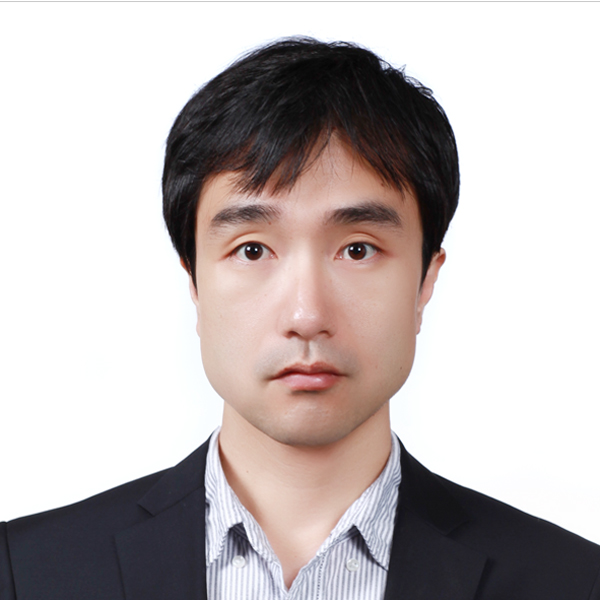
\includegraphics[width=1in,height=1.25in,clip,keepaspectratio]{sangho}
% \end{minipage}
% ~
\begin{minipage}{0.5\linewidth}
  Post-doctoral Research Associate \\
  Dept. of Computer Science \& Engineering \\
  \href{http://www.postech.ac.kr}{POSTECH} \\  
  Pohang, Republic of Korea
\end{minipage}
\begin{minipage}{0.5\linewidth}
  \begin{tabular}{ll}
    Phone:    & +82 54 279 2915 \\
    Fax:      & +82 54 279 1805 \\
    Email:    & {\tt sangho2@postech.ac.kr} \\
%               & {\tt sangho35.lee/@/gmail.com} \\
    Web: & {\tt https://hpc.postech.ac.kr/$\sim$sangho2} \\
  \end{tabular}
\end{minipage}

\section*{Education}

\begin{itemize}
  \item March 2008--February 2013: Ph.D. in Computer Science and Engineering, POSTECH
  \begin{itemize}
  \item \textbf{Detection and Prevention of Web Security Attacks Exploiting URL Redirection}
  \item Committee: Jong Kim (advisor), Sung Je Hong, Jangwoo Kim, Gary Geunbae Lee, Pil Joong Lee
  \end{itemize}
   % (GPA: 3.7/4.3).
  \item March 2006--February 2008: M.S. in Computer Science and Engineering, POSTECH
  \begin{itemize}
  \item \textbf{Redistributing Time-based Rights for Content Sharing in DRM}
  \item Committee: Jong Kim (advisor), Sung Je Hong, Pil Joong Lee
  \end{itemize}  
   % (GPA: 4.09/4.3).
  \item March 2002--February 2006: B.S. in Computer Engineering, Hongik University %(GPA: 4.3/4.5, Major: 4.48/4.5).
  \begin{itemize}
  \item GPA: 4.3/4.5 (total), 4.48/4.5 (major only)
  \end{itemize}  
\end{itemize}


% \section*{Thesis}
% \begin{itemize}
%  \item
%  Detection and Prevention of Web Security Attacks Exploiting URL Redirection,
%  Doctoral Thesis, Department of Computer Science and Engineering, POSTECH, 
%  February 2013. 
%  \begin{itemize}
%  \item Committee: Jong Kim (chair), Sung Je Hong, Jangwoo Kim, Gary Geunbae Lee, Pil Joong Lee
%  \end{itemize}
%  \item
%  Redistributing Time-based Rights for Content Sharing in DRM, 
%  Master's Thesis, Department of Computer Science and Engineering, POSTECH, 
%  February 2008.
%  \begin{itemize}
%  \item Committee: Jong Kim (chair), Sung Je Hong, Pil Joong Lee
%  \end{itemize} 
% \end{itemize}

\section*{Employment}
\begin{itemize}
  \item Post-doctoral Research Associate, POSTECH, from March 2013.
  \item Research Assistant, POSTECH, March 2006--February 2013.
\end{itemize}

\section*{Research Interests}
 %Information, Network, and System Security, Applied Cryptography
All aspects of computer security and privacy including Web and social network security, system security, mobile security, and applied cryptography
% Web and social network security, applied cryptography, network security, system security

\section*{Referred Publications}
% \section*{Selected Publications}

\subsection*{International Conference}
\begin{longtable}{@{}p{0.8in}p{5.4in}@{}}
  \textbf{NDSS'15} &  \myname, Hyungsub Kim, and Jong Kim, Identifying Cross-origin Resource Status Using Application Cache, 
  {\em Proceedings of Network and Distributed System Security Symposium ({NDSS})}, San Diego, California, USA, February 8--11, 2015. \\\\
  \textbf{ACSAC'14} & Hyungsub Kim, \myname, and Jong Kim, Exploring and Mitigating Privacy Threats of HTML5 Geolocation API, 
  \emph{Proceedings of Annual Computer Security Applications Conference (ACSAC)}, New Orleans, Louisiana, USA, December 8--12, 2014.\\\\
  \textbf{Oakland'14} & \myname, Youngsok Kim, Jangwoo Kim, and Jong Kim, Stealing Webpages Rendered on Your Browser by Exploiting GPU Vulnerabilities, \emph{ Proceedings of IEEE Symposium on Security and Privacy ({Oakland})}, San Jose, California, USA, May 19--21, 2014.\\\\
  {WISA'13} & Hayoung Lee, Taeho Kang, \myname, Jong Kim, and Yoonho Kim, Punobot: Mobile Botnet using Push Notification Service in Android, {\it Proceedings of International Workshop on Information Security Applications (WISA)}, Jeju Island, Korea, August 19--21, 2013.\\\\
  \textbf{WWW'13} & Jonghyuk Song, \myname, and Jong Kim, I Know the Shortened URLs You Clicked on Twitter: Inference Attack using Public Click Analytics and Twitter Metadata, \emph{Proceedings of International World Wide Web Conference ({WWW})}, Rio de Janeiro, Brazil, May 13--17, 2013.\\\\
  \textbf{NDSS'12} & \myname and Jong Kim, WarningBird: Detecting Suspicious URLs in Twitter Stream, \emph{Proceedings of Network and Distributed System Security Symposium ({NDSS})}, San Diego, California, USA, February 5--8, 2012.\\\\
  \textbf{RAID'11} & Jonghyuk Song, \myname, and Jong Kim, Spam Filtering in Twitter using Sender-receiver Relationship, \emph{Proceedings of International Symposium on Recent Advances in Intrusion Detection ({RAID})}, Menlo Park, California, USA, September 20--21, 2011.\\\\
  CCNC'11 & \myname and Jong Kim, A Batch Rekeying Time Decision Algorithm for IPTV Systems, {\it Proceedings of 8th IEEE Consumer Communications and Networking Conference (CCNC)}, Las Vegas, Nevada, USA, January 9--12, 2011.\\\\
  ISCC'10 & \myname, Heejin Park, and Jong Kim, A Secure and Mutual-profitable DRM Interoperability Scheme, {\it Proceedings of 15th IEEE Symposium on Computers and Communications (ISCC)}, Riccione, Italy, June 22--25, 2010.\\\\
  BMSB'08 & Yuna Kim, Jae Keun Park, Hong Jun Choi, \myname, Heejin Park, Jong Kim, Zino Lee, and Kwangil Ko, Reducing IPTV Channel Zapping Time based on Viewer's Surfing Behavior and Preference, {\it Proceedings of 2008 IEEE International Symposium on Broadband Multimedia Systems and Broadcasting (BMSB)}, Las Vegas, USA, Mar. 31--Apr. 2, 2008.
\end{longtable}

\subsection*{International Journal}
\begin{longtable}{@{}p{0.8in}p{5.4in}@{}}
  % COMSIS'15 & {\bf Sangho Lee}, Jong Kim, and Yoonho Kim, Preserving Source- and Sink-location Privacy in Sensor Networks, To appear in {\it Computer Science and Information Systems}.\\\\
  TDSC'15 & Jonghyuk Song, \myname, and Jong Kim, Inference Attack on Browsing History of Twitter Users using Public Click Analytics and Twitter Metadata, To appear in {\it IEEE Transactions on Dependable and Secure Computing} (SCIE).\\\\
  COMCOM'14 & \myname and Jong Kim, Early filtering of ephemeral malicious accounts on Twitter, 
  {\it Computer Communications} 54, 48--57, December 2014 (SCIE).\\\\
  TDSC'13 & \myname and Jong Kim, WarningBird: A Near Real-time Detection System for Suspicious URLs in Twitter Stream, {\it IEEE Transactions on Dependable and Secure Computing}, 10(3), 183--195, May-June 2013 (SCIE).\\\\
  COMCOM'13 & \myname and Jong Kim, Fluxing botnet command and control channels with URL shortening services, {\it Computer Communications} 36(3), 320--332, February 2013 (SCIE).\\\\
  COMML'12 & \myname, Jin Seok Kim, Sung Je Hong, and Jong Kim, Distance Bounding with Delayed Responses, {\it IEEE Communications Letters} 16(9), 1478--1481, September 2012 (SCI).\\\\
  JSS'12 & \myname, Hay-Rim Lee, Seungkwang Lee, and Jong Kim, DRMFS: A file system layer for transparent access semantics of DRM-protected contents, {\it Journal of Systems and Software} 85(5), 1058--1066, May 2012 (SCIE).\\\\
  IJIS'09 & \myname, Jong Kim, and Sung Je Hong, Redistributing time-based rights between consumer devices for content sharing in DRM system, {\it International Journal of Information Security} 8(4), 263--273, August 2009 (SCIE).\\\\
  JSS'09 & \myname, Jong Kim, and Sung Je Hong,  Security weakness of Tseng's fault-tolerant conference-key agreement protocol, {\it Journal of Systems and Software} 82(7), 1163--1167, July 2009 (SCIE).\\\\
\end{longtable}

% \section*{Under Review}
% \begin{itemize}
% \item \myname, Beumjin Cho$^*$, Meng Xu, Sangwoo Ji, Taesoo Kim, and Jong Kim, BreakUp: Preventing Cross-update Privacy Leaks on Android
% %, {\it Proceedings of 22nd ACM Conference on Computer and Communications Security (CCS)}, Denver, CO, USA, October 12--16, 2015.
% \item \myname, Hyungsub Kim$^*$, and Jong Kim, Inferring Web Privacy Through Remote Monitoring of Storage Usage
% %, {\it Proceedings of 22nd ACM Conference on Computer and Communications Security (CCS)}, Denver, CO, USA, October 12--16, 2015.
% \item Jonghyuk Song, \myname, and Jong Kim, CrowdTarget: Target-based Detection of Crowdturfing in Online Social Networks
% %, {\it Proceedings of 22nd ACM Conference on Computer and Communications Security (CCS)}, Denver, CO, USA, October 12--16, 2015.
% \item Jonghyuk Song, \myname, and Jong Kim, Identifying Users in Multiple Social Networks Through Reactions to Cross-site Posts
% %, {\it Proceedings of 20th European Symposium on Research in Computer Security (ESORICS)}, Vienna, Austria, September 21--25, 2015.
% \item \myname, Jong Kim, and Yoonho Kim, Preserving Source- and Sink-location Privacy in Sensor Networks, 
% %, To appear in {\it Computer Science and Information Systems} (SCIE).
% \item $^{*}$ Co-first authors
% \end{itemize}

% \section*{Thesis}
% \begin{itemize}
%  \item
%  Detection and Prevention of Web Security Attacks Exploiting URL Redirection,
%  Doctoral Thesis, Department of Computer Science and Engineering, POSTECH, 
%  February 2013. 
%  \begin{itemize}
%  \item Committee: Jong Kim (chair), Sung Je Hong, Jangwoo Kim, Gary Geunbae Lee, Pil Joong Lee
%  \end{itemize}
%  \item
%  Redistributing Time-based Rights for Content Sharing in DRM, 
%  Master's Thesis, Department of Computer Science and Engineering, POSTECH, 
%  February 2008.
%  \begin{itemize}
%  \item Committee: Jong Kim (chair), Sung Je Hong, Pil Joong Lee
%  \end{itemize} 
% \end{itemize}

\section*{Patents}
\begin{itemize}
  \item
 Jong Kim, \myname, and Heejin Park,
 Methods and apparatuses for providing DRM interoperability,
 Registration, USA, 8,386,799,
 February 2013. 
 \item
 \myname and Jong Kim,
 Method of distributing time of using contents between personal devices and system based on the same,
 Registration, Korea, 10-0951792,
 April 2010.
  \item
 Heejin Park, Jong Kim, and \myname,
 Method and apparatus for rights-preserving interoperability in DRM,
 Registration, Korea, 10-0942992
 February 2010. 
\end{itemize}

\section*{Projects}

\begin{itemize}
 \item January 2010--December 2011: Research on the context-aware privacy protection platform for mobile devices, ITRC-CMEST
 \item February 2010--April 2011: Research on the vulnerabilities of smart TVs, Samsung Electronics
 \item March 2006--December 2009: Research on the DRM middleware for mobile devices, ITRC-CMEST.
 \item March 2007--November 2008: Research on the security of IPTV systems, Contron and Alticast.
 \item September 2007--February 2008: Survey on the sensors and industrial applications of USN, SECUI.COM.
 \item March 2006--October 2006: Research on the detection rule optimization to improve IDS engine, NSRI.
\end{itemize}

% \section*{Academic Experience}

% \begin{itemize}
%  \item Teaching Assistant, Data Structures, POSTECH, Fall 2007.
% \end{itemize}

\section*{Honors and Awards}

\begin{itemize}
 \item Runner-up Prize, Evaluation of ITRC Support Program, 2013.
 \item Good Paper Award, KIISC Winter Conference, 2008.
 \item Good Paper Award, KIISE Fall Conference, 2007.
 % \item Best Grade Scholarship, Hongik University, from 2002 to 2006.
\end{itemize}

\section*{Professional Activities}

\begin{itemize}
% \item External reviewer for WWW, ICDCS, NDSS, IEEE Trans. Dependable and Secure Computing, IEEE Communications Letters, and Wiley Security and Communication Networks
\item External/sub reviewer for ICDCS, WWW, NDSS, IEEE Communications Letters, IEEE Trans. Dependable and Secure Computing, Security and Communication Networks, ACM Trans. Embedded Computing, Journal of Computing Science and Engineering
% \item Student Member of IEEE
\end{itemize}

\section*{Talks}
\begin{itemize}
\item Detection of Suspicious URLs with Conditional Redirection, {\it Invited Seminar}, ETRI, Daejeon, Korea, March 17, 2015.
\item Privacy Leakage from GPU Exploits, {\it Invited Seminar}, KAIST, Daejeon, Korea, March 10, 2015.
\item Identifying Cross-origin Resource Status Using Application Cache, {\it 22nd Network and 
    Distributed System Security Symposium (NDSS)}, San Diego, California, USA, February 9, 2015.
\item Web and Browser Security: Attack and Defense, {\it Invited Seminar}, UNIST, Ulsan, Korea, January 21, 2015.
\item Stealing Webpages Rendered on Your Browser by Exploiting GPU Vulnerabilities, {\it 35th IEEE Symposium on Security and Privacy (Oakland)}, San Jose, California, USA, May 19, 2014.
% \item Distributed certificate authority scheme with weighted secret sharing for mobile ad-hoc networks, {\it 4th International Conference on Network of the Future (NoF)}, Pohang, Korea, October 24, 2013.
\item Spam and Browsing Privacy Problems on Twitter, {\it Invited Seminar}, KAIST, Daejeon, Korea, May 27, 2013.
\item WarningBird: Detecting Suspicious URLs in Twitter Stream, {\it 19th Network and 
    Distributed System Security Symposium (NDSS)}, San Diego, California, USA, February 8, 2012.
\item A Batch Rekeying Time Decision Algorithm for IPTV Systems, {\it 8th IEEE Consumer
    Communications and Networking Conference (CCNC)}, Las Vegas, Nevada, USA, January 11, 2011.
\item A Secure and Mutual-profitable DRM Interoperability Scheme, {\it 15th IEEE Symposium on
    Computers and Communications (ISCC)}, Riccione, Italy, June 22, 2010.
% \item Program-value aware Adaptive Group-key Rekeying for IPTV, {\it KIPS Fall Conference}, Seoul,
%   Korea, November 15, 2008.
% \item Efficient Fault-tolerant Conference-key Agreement based on ID-based Tripartite Key Agreement
%   Protocol, {\it KIISE Fall Conference}, Busan, Korea, October 27, 2007.
% \item DRM-enabled Adaptive User Domain using Time-block Redistribution, {\it 5th Joint Workshop
%     between Security Research Labs in Korea and Japan}, Hakodate, Japan, August 4, 2007.
% \item Controlled Content Sharing based on Time-block Distribution in DRM, {\it 4th Joint Workshop
%     between Security Research Labs in Korea and Japan}, Pohang, Korea, January 29, 2007.
\end{itemize}

% \section*{Skills}
% \begin{itemize}
% \item Programming: C, C++, Python, Java, HTML, JavaScript, PHP, CUDA, and OpenCL
% \item Language: Korean (native), English (advanced), and Japanese (beginner)
% \end{itemize}

% \begin{minipage}{0.15\linewidth}
% \includegraphics[width=\linewidth]{sangho2}
% % 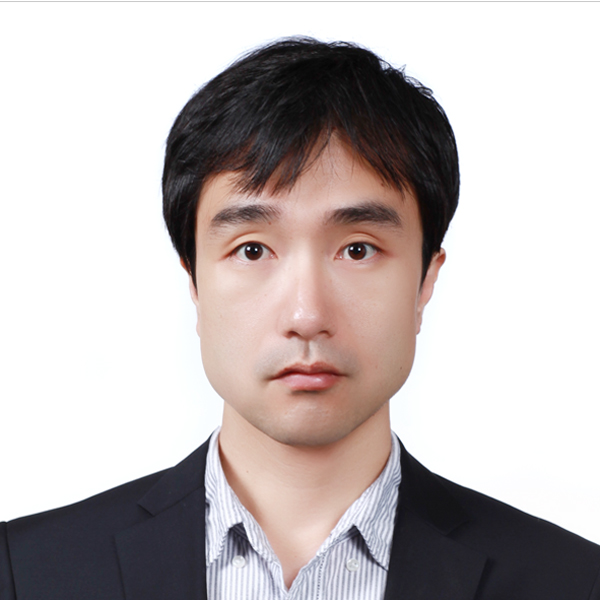
\includegraphics[width=1in,height=1.25in,clip,keepaspectratio]{sangho}
% \end{minipage}
% ~
% \begin{minipage}{0.5\linewidth}
%   Post-doctoral Research Associate \\
%   Dept. of Computer Science \& Engineering \\
%   \href{http://www.postech.ac.kr}{POSTECH} \\  
%   Pohang, Republic of Korea
% \end{minipage}
% \begin{minipage}{0.5\linewidth}
%   \begin{tabular}{ll}
%     Phone:    & +82 54 279 2915 \\
%     Fax:      & +82 54 279 1805 \\
%     Email:    & {\tt sangho2@postech.ac.kr} \\
% %               & {\tt sangho35.lee/@/gmail.com} \\
%     % Homepage: & {\tt https://hpc.postech.ac.kr/$\sim$sangho2} \\
%   \end{tabular}
% \end{minipage}

% \section*{References}
% \noindent
% \textbf{Jong Kim}\\
% Professor\\
% Department of Computer Science and Engineering\\
% POSTECH\\
% Nam-gu, Pohang-si, Gyeongsangbuk-do, Korea\\
% +82 54 279 2257\\
% {\tt jkim@postech.ac.kr}\\

% \noindent
% \textbf{Jangwoo Kim}\\
% Associate Professor\\
% Department of Computer Science and Engineering\\
% POSTECH\\
% Nam-gu, Pohang-si, Gyeongsangbuk-do, Korea\\
% +82 54 279 2390\\
% {\tt jangwoo@postech.ac.kr}\\

% \noindent
% \textbf{Kyong Hoon Kim}\\
% Associate Professor\\
% Department of Informatics\\
% Gyeongsang National University\\
% Gajwa-dong, Jinju-si, Gyeongsangnam-do, Korea\\
% +82 55 751 1375\\
% {\tt khkim@gnu.ac.kr}

% \begin{minipage}{0.33\linewidth}
% {Prof. Jong Kim}\\
% POSTECH\\
% % Nam-gu, Pohang-si\\
% Pohang, Gyeongbuk, Korea\\
% +82 54 279 2257\\
% {\tt jkim@postech.ac.kr}
% \end{minipage}
% ~
% \begin{minipage}{0.33\linewidth}
% {Prof. Jangwoo Kim}\\
% POSTECH\\
% % Nam-gu, Pohang-si\\
% Pohang, Gyeongbuk, Korea\\
% +82 54 279 2390\\
% {\tt jangwoo@postech.ac.kr}
% \end{minipage}
% ~
% \begin{minipage}{0.33\linewidth}
% {Prof. Kyoung Hoon Kim}\\
% Gyeongsang National University\\
% % Gajwa-dong, Jinju-si\\
% Jinju, Gyeongnam, Korea\\
% +82 55 751 1375\\
% {\tt khkim@gnu.ac.kr}
% \end{minipage}
% \begin{minipage}{0.33\linewidth}
% Dr. Jin Seok Kim\\
% Agency for Defense Development\\
% Jinhae-gu, Changwon-si\\
% Gyeongsangnam-do, Korea\\
% +82 55 540 6218\\
% {\tt treasure@add.re.kr}
% \end{minipage}

\bigskip

% Footer
\begin{center}
  \begin{footnotesize}
    Last updated: \today \\
    \href{\footerlink}{\texttt{\footerlink}}
  \end{footnotesize}
\end{center}

\end{document}
